\documentclass[12pt]{report}
%\documentclass[12pt,twoside]{report}
% \documentclass{article}
\usepackage{amssymb}
\usepackage{algpseudocode}
\usepackage{algorithm}
\usepackage{setspace}
\usepackage{graphicx}
\graphicspath{ {./images/} }
\usepackage{hyperref}
\usepackage{siunitx}
\usepackage{amsmath}
\usepackage{caption}
\usepackage{subcaption}

\hypersetup{
    colorlinks=true,
    linkcolor=blue,
    filecolor=magenta,
    urlcolor=cyan,
}

\title {Ranking Loss Surrogates \\[1ex] \large MSc Thesis}
% Commenting out another way to write the title.
% \title{MSc Thesis - Ranking Loss Surrogates}

\author{
        Abdus Salam Khazi [
        \href{mailto:abdus.khazi@students.uni-freiburg.de}
                {Email} ]\\ \\
        \href{https://github.com/abduskhazi/ranking-loss-surrogates.git}
                {Github Repository} \cite{github_repository} \\ \\
        Supervisors:
        \begin{tabular}{ll}
             JProf. Josif Grabocka \&
			Sebastian Pineda
		\end{tabular}
       }

\begin{document}

\pagenumbering{gobble}


\maketitle
\date{}

\newpage
\pagenumbering{roman}
\begin{abstract}

Abstract goes here

\end{abstract}

\newpage

\tableofcontents
\newpage
\newpage

\pagenumbering{arabic}

\chapter{Introduction}

The performance of any machine learning model is sensitive to the hyper-parameters used during the model training. 
Instead of using a new model type, it is more helpful to tune the hyper-parameters of an existing model to improve its performance.
Learning the best hyper-parameter for an ML model is called, Hyperparameter optimization (HPO in short).
This thesis studies various existing approaches to HPO and proposes a new idea for the same using the concept of ranking.
The proposed idea in this thesis is called \textbf{HPO using Ranking Loss Surrogates}. 
The results obtained using this model are compared against the state-of-the-art results obtained using models like FSBO,  RGPE,  TAF, and others. 

\section{Problem Definition - HyperParameter Optimization}
To find out the best hyper-parameter for any machine learning model $m$, we must first quantify a given hyper-parameter configuration $\textbf{x}$ by a real-valued number $v \in \mathbb{R}$.
If we define that
$$
\textbf{x}_1 \succ  \textbf{x}_2 \iff v_{\textbf{x}_1} < v_{\textbf{x}_2}
$$
then HPO can be defined mathematically by an abstract function, say,  $f(\textbf{x}) \mapsto \mathbb{R}$ as
$$
     \underset{\rm \textbf{x}}{\rm argmin}  f(\textbf{x}) \;\;\;  \forall \textbf{x} \in \mathbb{S}
$$
where $\mathbb{S}$ is the hyper-parameter search space.

This function $f(\textbf{x}) \mapsto \mathbb{R}$ is evaluated in the following chronological steps:
\begin{enumerate}
\item Using a given hyper-parameter configuration $\textbf{x}$,  we train our model $m$ to obtain the model $m^{trained}_\textbf{x}$. It consists of learning the parameters of our model, E.g. learning the weights and biases of a Deep Neural Network.
We use the training data to learn this model.
\item The validation data is passed through $m^{trained}_\textbf{x}$ to obtain the required results.
These results are evaluated based on an evaluation criterion '$\textrm{eval}$'. This criterion is different for different problems, e.g. Regression, Classification, etc.
The result of this evaluation is a real-value that gives a score for the configuration $\textbf{x}$.
\end{enumerate}

Hence the function $f(\textbf{x}) \mapsto \mathbb{R}$ can be written as 
$$
\textrm{eval}(m^{trained}_\textbf{x} (\textrm{Data}_\textrm{val})) \mapsto \mathbb{R}
$$

Finally, the HPO problem can be defined using the following equation:
$$
\underset{\rm \textbf{x}}{\rm argmin} \;\; \textrm{eval}(m^{trained}_\textbf{x} (\textrm{Data}_\textrm{val})) \mapsto \mathbb{R}   \;\;\;  \forall \textbf{x} \in \mathbb{S}
$$

\label{ProblemOverviewlabel}
\section{Optimization Constraints}

Hyper-parameter optimization is different from other optimization methods because it has different constraints.
It is because of the peculiar properties of the hyper-parameter search spaces.
Finding out the correct hyper-parameter setting is generally not feasible using a brute-force approach (trying out all possible combinations of hyper-parameters) because the search space itself has many dimensions, and the search space may be continous.
More specifically,  some of the important constraints of this optimization problem are:

\begin{enumerate}
\item The evaluation of a given HPO configuration is computationally expensive.
\item It is a non-convex optimization problem.
\item The process of getting $m^{trained}_\textbf{x}$ from $m$ is stochastic hence the value $v_{\textbf{x}}$ is noisy.
\item Some dimensions have conditional constraints. The values of some dimensions may depend on the values of others. For example, the number of neurons in layer 3 only makes sense if we have 3 or more layers in a neural network.
\item The search space is hybrid in terms of continuity. Some of the dimensions (variables) may be continuous, while others may be discrete.
Using a gradient method is hence not trivial.
\end{enumerate}


\section{Overview}
This sections contains the overview of the paper and how the thesis report is organised.


\chapter{Literature Review}
To deal with the constraints of HPO problems, researchers have used different strategies for developing HPO algorithms and models.
Some of the straightforward methods include
\begin{itemize}
\item Manual Search
\item Grid Search
\item Random Search
\end{itemize}


Manual Search in the HPO search space is feasible when we have expert knowledge of the problem and the given model. 
The idea is to select configurations step by step by observing the results obtained
so that we do not waste computation time evaluating similar configurations through intuition.
This approach may be helpful for small models with lesser constraints.
However, as the HPO search space becomes very large or conditional constraints become too complex, the selection of configurations becomes more and more difficult.
Hence a more systematic and automated approach is more practical.

Grid search is a more systematic approach in which we divide the search space into grid points similar to ones in a Euclidean graph.
Let there be $m$ dimensions in the search space $\mathbb{S}$. Let the selected number of values for each dimension be $n_1, n_2, ... n_m$. In the case of a discrete variable, the selected values will be a subset of the possible values, whereas, in the case of a continuous variable, we need to select the values based on a selected granularity.
The cross-product of the selected subsets gives us the configurations to be evaluated. Hence, the number of configurations to evaluate will be $n_1 * n_2 * ... n_m$.
The number of configurations we need to evaluate in this approach becomes a big issue for this method as the dimensions of the search spaces increase.
Hence this approach becomes intractability for large search spaces.

\begin{figure}[htb]
  \centering
    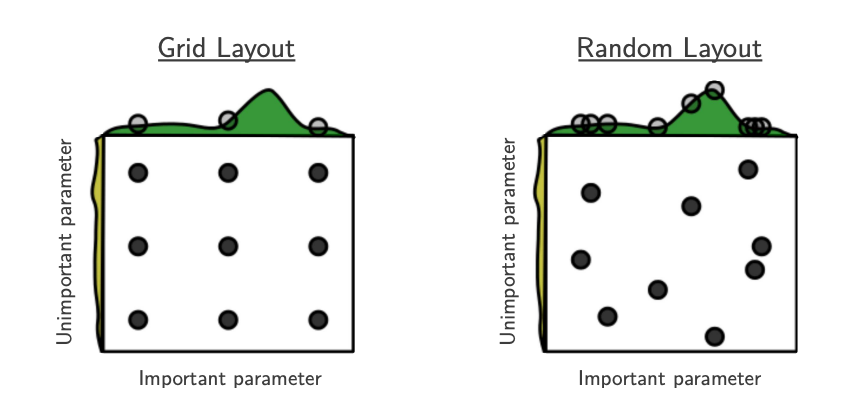
\includegraphics[scale=0.8]{images/rsgsexample}
    \caption{Illustrates Grid search and Random search in the case where 2 parameters are not equally important.  Adpated from~\cite{rshpoarticle}.}
    \label{fig:rshpofig}
\end{figure}

One issue with the Grid Search approach is that we assume that all dimensions in the HPO search space are equally important. It is not the case in many HPO problems.  The Grid layout in Figure~\ref{fig:rshpofig}(left) shows illustrates this.  For example, the learning rate in deep neural networks is much more important than many other parameters. If dimension $p$ is the most important in the search space, then it makes sense to evaluate more values of $p$. Random Search helps us solve this problem. 
The Random layout in Figure~\ref{fig:rshpofig}(right) illustrates this. 
Hence Random Search can be used as a trivial baseline for comparing other HPO models.

One advantage of these methods is that there are no restrictions on the HPO search spaces. Hence, they are suitable for any HPO problem at hand.
On the other hand, these methods are non-probabilistic.
Hence they cannot deal with noisy evaluations of the HPO configuration well.
Moreover, these methods are computationally expensive. The reason is that they do not use surrogate evaluators and hence train and evaluate the whole model.
Also, these search methods give us optimal HPO configurations only by chance.

In the remainder of this section, we discuss some sophisticated probabilistic models for doing HPO that use surrogates to reduce computational costs.

\section{Bayesian Optimization}
Bayesian optimization tries to solve both computational costs and noisy evaluations of our objective function (section 1).
It does this by building a model of the HPO objective function. This model is called a surrogate function.
Bayesian optimization uses known evaluations as its data to build the surrogate model. The data is of the form {x, f(x)} pairs.
The surrogate model is a probabilistic model. Hence, it also learns about the noise in the evaluations of the objective function.

The core procedure of the optimization process is the following:
\begin{itemize}
\item From known data $D = {(x_1, f(x_1)), (x_2, f(x_2)), (x_3, f(x_3)) .... }$, build a probabilistic model that learns the mean and variance of the objective function
\item Use the surrogate to sample the next best HPO configuration x'. Evaluate f(x')
\item Append (x', f(x')) to D and repeat the process.
\end{itemize}

The above process repeats till the computational resources are finished (here time) or we find an acceptable HPO configuration.
This procedure is also called SMBO (Sequential model-based Optimization).
The procedure alternates between collecting data and fitting the model with the 
collected data~\cite{SMBOPaper}.

There are two essential components of Bayesian optimization:

\begin{itemize}
\item Probabilistic model of the objective function
\item The acquisition function
\end{itemize}

There are many probabilistic models such as Random Forests, Gaussian Processes, Tree parson Estimators, etc.
But for the purpose of this thesis, we briefly mention Random forests and discuss in-depth the Gaussian processes.

\subsection{Probabilistic models}
\subsubsection{Random Regression Forest}
     The core idea of this model is to train a Random Regression Forest, using the known data as in any SMBO procedure~\cite{SMBOPaper}.
Random regression forests are an ensemble of regression trees. 
This property is used to our advantage to predict the mean and the variance. 
The mean of the prediction of all the trees is the mean of the surrogate model.
The variance in the prediction of all trees is the variance of the surrogate model.

   The advantages of this model are
   \begin{itemize}
   \item It can handle both continuous and discrete variables trivially without any modifications to the model.
The data splitting during training is done using any variable be it discrete or continuous.
	\item It can handle conditional variables, unlike Gaussian processes, by making sure that data is not split based on a variable till it is guaranteed that no conditionality is broken by the split.
   \end{itemize}


\subsubsection{Gaussian Process Regression}

Gaussian processes~\cite{GPTutorial} are predictive machine learning models that work well with few data points (or data pairs). 
They are inherently capable of modeling uncertainty.
Hence, they are used widely in problems such as hyperparameter optimization, where uncertainty estimation is essential.
In this section, we briefly explain the Gaussian process regression intuitively.

Before we proceed,  we need to understand normal (Gaussian) distributions. 
Consider a scalar random variable $X$ that is distributed normally  (a.k.a Gaussian distribution) around a mean $\mu$ with a variance of $\sigma^2$.
The following equation defines the probability density function (PDF) of $X$: 
$$
P_X(x) = \frac{1}{\sqrt[2]{2\pi}\sigma}\exp\left(- \frac{(x - \mu)^2}{2\sigma^2}\right)
$$
Here, $X$ represents the random variable, and $x$ represents an instance of the variable~\cite{GPTutorial}.
In this case,  the mean $\mu$,  variance $\sigma^2$, and any sample $x$ are all scalars.

If the random variable $\textbf{X}$ is a vector in $\mathbb{R}^d$ where $d \in I^{+}$,  then each component of the vector can be considered as a random variable.
In this case the mean $\boldsymbol{\mu} \in \mathbb{R}^d$ whereas variance, represented by $\Sigma$, is in the $R^{d \times d}$ space.
It is because the variance of all components in any valued vector random variable $\textbf{X}$ should contain the following two types of variance
\begin{itemize}
\item Variance of a vector component w.r.t itself.
$d$ diagonal values of the matrix $\Sigma$ represent this variance.
\item Variance of each vector component w.r.t all other components. These variances are represented by the upper/lower triangular values in the matrix $\Sigma$.
\end{itemize}
The matrix $\Sigma$, also known as the Covariance matrix, thus has all values necessary to represent the variance of any vector-valued random variable.


The probability density function of a vector valued variable $\textbf{X} \in \mathbb{R}^d$ with a mean $\boldsymbol{\mu}$ and covariance matrix $\Sigma$ is given by~\cite{MITMLBook}:

$$
\mathcal{N}(\textbf{x} | \boldsymbol{\mu},  \Sigma) = 
\frac{1}{(2\pi)^{\frac{d}{2}} |\Sigma|^{\frac{d}{2}}}
\exp\left( - \frac{1}{2} (\textbf{x} - \boldsymbol{\mu})^T  \Sigma^{-1}   (\textbf{x} - \boldsymbol{\mu}) \right)
$$
This equation defines the PDF of a multivariate normal distribution.

The core idea used in the Gaussian processes is that functions can be considered as vectors of infinite dimensions.
Consider any function $f$ that has a domain $\mathbb{R}$.
If $f$ is considered to be a vector in $\mathbb{R}^{\infty}$,
then each point $i \in \mathbb{R}$  can be represented by a component $f_i$ of the function $f$.
A function,  hence,  is nothing but a sample from $\mathbb{R}^{\infty}$.
Unfortunately, functions sampled from $\mathbb{R}^{\infty}$ are too general and not useful by themselves.

The idea of Gaussian processes is to sample smooth functions from $\mathbb{R}^{\infty}$.
In any smooth function $f$, if any point $g$ is close to $x$ in the domain of $f$, then $f(g) \approx f(x)$.
It is mathematically represented by the following equation:
$$
\lim_{\delta x \to 0} f_{x + \delta x} \approx f^{+}_x  \;\; \textrm{and} \;\; 
\lim_{\delta x \to 0} f_{x - \delta x} \approx f^{-}_x 
$$
$$\;\; \textrm{where} \;\; \delta x > 0 \;\; \textrm{and} \;\; x, \delta x \in \mathbb{R}
$$
The above definition is nothing but the definition of a smooth function in terms of vector notation. 
Moreover, nearby components of $f$ "vary" similarly w.r.t each other.
These properties can be naturally encoded using a covariance matrix.
Hence, we obtain smooth functions if we sample them from a multivariate normal distribution with the required covariance matrix.
The Gaussian process restricts the function sample space to a multivariate normal distribution.

The similarity between 2 points in a domain is defined by a function called \textbf{kernel} in Gaussian processes.
Using this kernel function, the values in the required covariance matrix are populated.
The smoothness of the sampled function $f$ is controlled by the kernel in the GP process.
Formally kernel $k$ is defined as,
$$
k(\textbf{x}, \textbf{x'}) \mapsto \mathbb{R}
$$

Here, $\textbf{x}, \textbf{x'}$ belong to a domain in the most abstract sense.
For example,  when the input domain is a euclidean space,  $\textbf{x} \in \mathbb{R}^{\mathbb{I}^+}$.

\subsection{Acquisition functions}


Due to the robustness of the GP process, we use this as one of the baselines in our thesis.
\section{Deep Ensembles}
One way to do Hyper Parameter Optimization is by using 
Uncertainty prediction is the key in the paper~\cite{DeepEnsemblePaper}.

\section{RGPE}
This section is necessary because our model performs similar to this

\section{TAG}
Some other model if also necessary and you mention this in your report.

\section{Deep Kernel Learning}

\section{Ranking Loss functions}
Types of ranking losses
\subsection{Pair wise ranking losses}
\subsection{...}
\subsection{List wise ranking losses}


\chapter{Baseline Implementations}
\section{Dataset}
This section defines the requirement of the dataset and why meta data sets are important
\subsection{Models used}
\subsection{Meta dataset}
Various search spaces sizes
\subsection{HPO\_B Dataset}
How HPOB datasets is organised.

\section{Deep Ensemble}
\subsection{Requirement of restarting training}
We find in our experiments that the deep ensemble performance much better in our HPO cycle when we train it from scratch at every acquisition step.
This is counter intuitive because an already trained model will converge to a local optima quickly.
The reason for this performance however is that the model gets biased towards the points that are observed in the beginning.
Lets say we have 2 models 
\begin{itemize}
\item $\textrm{DE}_{\textrm{restart}}$ which always restarts training at every acquisition step
\item $\textrm{DE}_{\textrm{reuse}}$ which uses the previously trained model for subsequent training of the optimization cycle.
\end{itemize}

The following figures show the number of times each observed data points is used for training at 25th 50th and 100th optimization cycle.
All the data is used in the optimization cycle as the amount of data is very less.
Hence the diagrams are scaled with the number of epochs.

The heavy bias that you can see in the figures is actually not intended.
This is because all observations should be treated equally in any training/fine-tuning step.

Create Bias diagram...

The second reason is that we may not be able to get out of the local minima.
Support using a diagram.

\section{Few Shot BO: Deep Kernel Learning}

\chapter{Proposed Idea: Ranking Loss Surrogates}

The search spaces that have less data need more uncertainty
The search spaces having more data need less uncertainty

We use list wise ranking losses because they have been found to be more efficient

\section{case study: Sorting}

\section{Scoring function analysis}
\subsection{Scoring function range}

\section{Optimization cycle}
\subsection{Meta training}
\subsection{Fine tuning}

\section{Loss function implementation}
The loss function used is listMLE
the implementation is done by removing to element check comments
The latest implementation is used due to its efficiency otherwise it is the same. (note)

\subsection{Weighted Loss}
Weighting becomes important because we are doing fine tuning at every step.
Show the equation for weighting
Used log weighting because 
Advantages:
Can be used to select best n configs and then evaluated at random based on the ranks. This is not as trivial to get in otherplaces. So there is an amount of parallelism that can be built it.

Parallelisation of elements is possible.

show the architecture of with only scorer
\section{Use of Deep Sets}
why are deep sets important. 

Architectecture with deep sets.. Image

\section{Uncertainty implementation}
Mention about the requirement to use Module list.
Show the new architecture.

\section{Advantages and Limitations}
Compare this loss function and method with other base lines..


\chapter{Experiments and Results}

experiment and results
protocol
data split…

First show the resutls of implementation of GP (M = 5 and M =10 )
Benchmark this...

Next with DKT (Benchmark this)

Next show the best results obtained by architecture.

\section{Evaluation}
\subsection{Testing}
\subsection{Ablation}

show the results of raw without deep set.

Next show different strategies used for building the ranking loss model one step at a time.
First with only scorer.
then with deep set.
Then with raw deep set
fine tuning and deep set
adding uncertainty

Checking the early stop and hypothesing why is was wrong.

box plot variation of each of the scorers... for 1 or more data sets?

what about training independently , this requires normalization. as explained by sebastian.

\chapter{Conclusion}

\section{Further work}
Further study required with other baselines that deal with ranking loss.

\section{Conclusion}

\bibliographystyle{plain}
\bibliography{references}
\pagenumbering{roman}

\appendix
% \chapter*{Appendices}
\chapter{More information}
This thesis was completed in the representation learning lab of Albert-Ludwig-Universität Freiburg.  (Figure~\ref{fig:UniLogo})

\begin{figure}[htb]
  \centering
    \includegraphics[scale=0.35]{images/logo}
    \caption{Logo: Albert-Ludwig-Universität Freiburg}
    \label{fig:UniLogo}
\end{figure}

\end{document}

